\documentclass[t,pdflatex]{beamer}
\usepackage[utf8]{inputenc}

%\usetheme{Frankfurt}

\title{Learning Breakout using NEAT}
\author{James~T.~Murphy~III\thanks{\url{jamesmurphy@math.utexas.edu}}\and{}Skyler~Thomas\thanks{\url{skylerthomas0@gmail.com}}}
\institute{The University of Texas at Austin}
\date\today

\begin{document}
\section{Title}

    \begin{frame}

        \titlepage

    \end{frame}

\section{Introduction}
    \begin{frame}

        In 2015, YouTuber SethBling trained a neural network to successfully beat the first level of Super Mario World [2].
        \frametitle{A neat application of a neat algorthim}
        \begin{figure}
            \centering
            
\includegraphics[width=.54 \textwidth]{mario.png}
        \end{figure}

        This was done using the Neural Evolution of Augmenting Technologies algorithm (NEAT) from the 2002 paper by Stanley and Mikkulainen [1].

    \end{frame}

    \begin{frame}

        \frametitle{NEAT, the algorithm}
        NEAT is a type of genetic algorithm that follows the biological metaheuristics of ``fitness begets evolution''.
        \begin{enumerate}
            \item Model neural network nodes and weights as genes.
            \item Randomly mutate genomes (add/delete node, add/delete connection, change connection weight,  etc.).
            \item Rank individuals by fitness.
            \item Allow best performing to mate using genetic crossover algorithm.
            \item Repeat until fitness threshold is reached.
        \end{enumerate}

    \end{frame}

        \begin{frame}

            \frametitle{Breakout (AKA BrickBreaker)}
        \begin{figure}
        \centering
        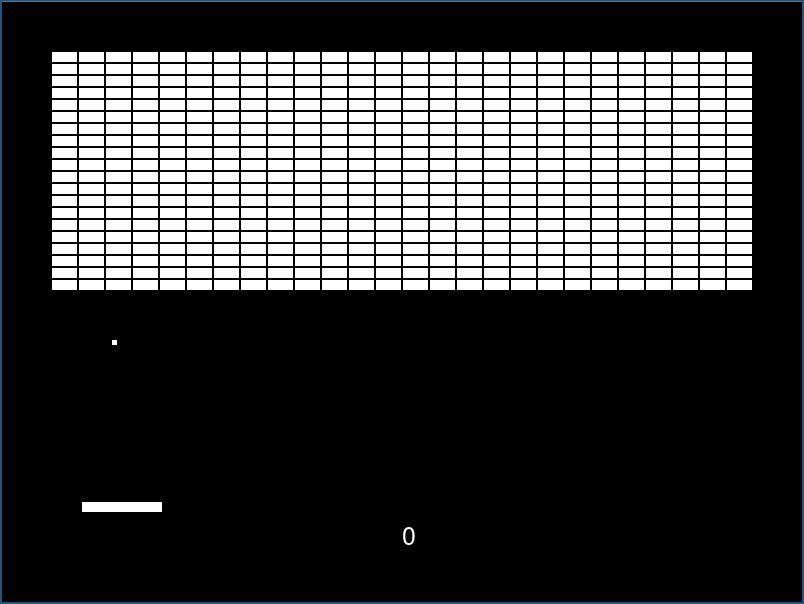
\includegraphics[width=.54 \textwidth]{breakout.png}
        \end{figure}

        We use the NEAT algorithm to train a network to play Breakout.
        The fitness of a genome is it's final score (out of 520) after playing a game of Breakout.

    \end{frame}

\section{Results}

    \begin{frame}

        \frametitle{Results}
        Qualitatively, it appears there are three eras:
        \begin{enumerate}
            \item Pre-ball-tracking era: The network does nothing or makes small and arbitrary movements.
            \item Ball-tracking era: It is apparent the paddle is tracking the ball, but it may make mistakes or infinite loop without clearing some remaining blocks.
            \item Aiming era: The network actively moves to and aims the ball to clear all 520 blocks.
        \end{enumerate}

        \pause{}
        Demo time!

    \end{frame}


    \begin{frame}

        \frametitle{Results}
        \begin{figure}[h!]
            \centering
            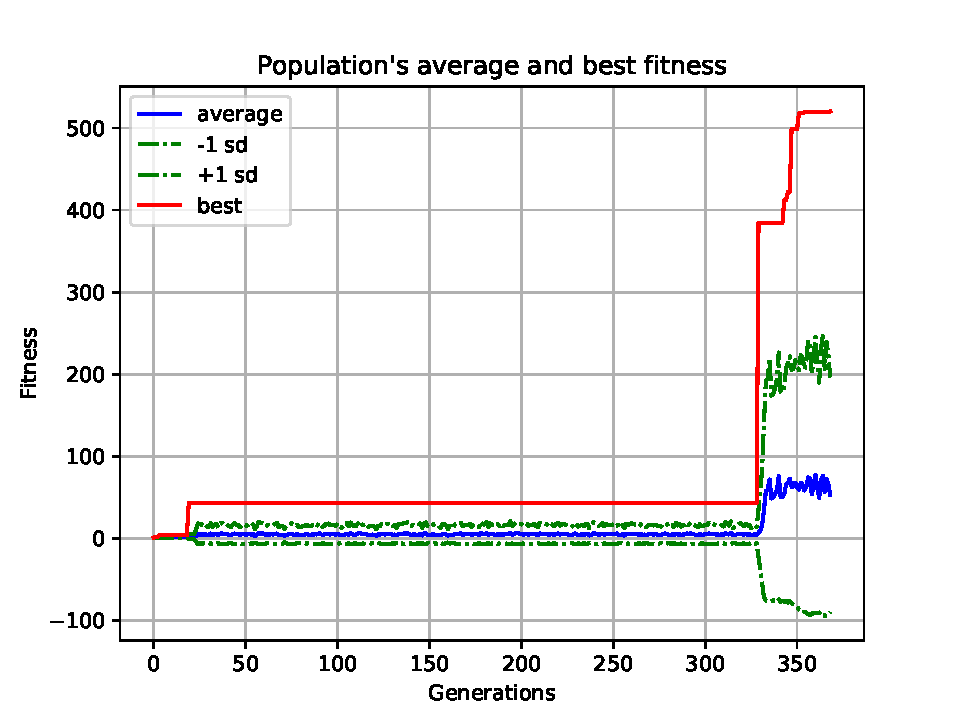
\includegraphics[width=.7 \textwidth]{avg_fitness.pdf}
            \caption{\textit{A successful training experiment.} 
                Generations of 200 individuals took an average time of 2.835 sec to evaluate on an
                Intel Core i7-4790K @ 4.00GHz in parallel on 6 cores. Total runtime $\approx$ 17.5 minutes.}
        \end{figure}

    \end{frame}

    \begin{frame}
        \frametitle{The winning network}
        The most fit network is extremely simple.
        It has no hidden nodes and only a few connections.
        \begin{figure}[h!]
            \centering
            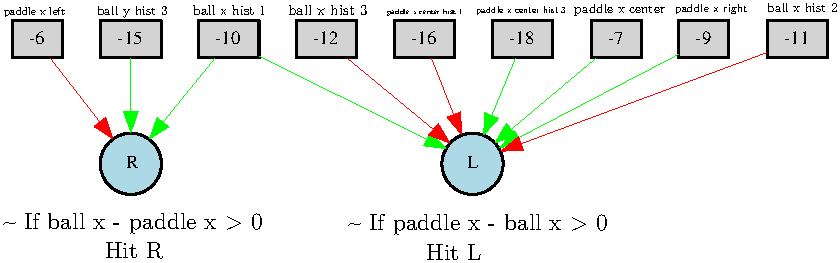
\includegraphics[width=1\textwidth]{winner_net_graph_annotated.pdf}
       \end{figure}
       This network is far too small to have memorized a sequence of inputs, it's actually tracking the ball.
    \end{frame}

\section{Discussion}

        \begin{frame}

        \frametitle{Discussion}
         \begin{itemize}
             \item Full board information too many inputs for success.
             \item Needed to give histroy of ball location for success.
             \item Needed to train with deterministic initial condition.
             \item Training prone to stagnation in a local maximum fitness.
             \item Success is \emph{very} sensitive to tiny changes in hyperparameters.
             \item Originally attempted to do Tetris, which was too complicated for NEAT with the current setup.
         \end{itemize}

    \end{frame}

        \begin{frame}

        \frametitle{Future}
        \begin{itemize}
            \item Change setup:
                \begin{enumerate}
                    \item Randomly generate initial board.
                    \item Make score based on 5 seconds of gameplay instead of full game.
                    \item Optionally, make score weighted by the amount of time it takes to achieve it to encourage clearing blocks \emph{quickly}.
                \end{enumerate}
            \item Compare NEAT vs.\ other evolutionary algorithms vs.\ non-evolutionary algorithms like Deep Q-learning.
        \end{itemize}


    \end{frame}

    \section{References}

    \begin{frame}
        \begin{thebibliography}{10}
        \beamertemplatearticlebibitems{}

%        \bibitem{neatpython}
%        CodeReclaimers.
%        \newblock Neat-python.
%        \newblock \url{https://neat-python.readthedocs.io}, August 2017.

%        \bibitem{stanley2002efficient}
%        K.~O. Stanley and R.~Miikkulainen.
%        \newblock Efficient reinforcement learning through evolving neural network
%          topologies.
        %\newblock In {\em Proceedings of the 4th Annual Conference on Genetic and
        %  Evolutionary Computation}, pages 569--577. Morgan Kaufmann Publishers Inc.,
        %  2002.

        \bibitem{stanley2002evolving}
        [1] K.~O. Stanley and R.~Miikkulainen.
        \newblock Evolving neural networks through augmenting topologies.
        \newblock {\em Evolutionary computation}, 10(2):99--127, 2002.

        \bibitem{sethbling2015}
        [2] SethBling.
        \newblock Mari/o machine learning for video games.
        \newblock \url{https://www.youtube.com/watch?v=qv6UVOQ0F44}, June 2015.

        \bibitem{mnih2013playing}
        [3] V.~Mnih, K.~Kavukcuoglu, D.~Silver, A.~Graves, I.~Antonoglou, D.~Wierstra, and
          M.~Riedmiller.
        \newblock Playing atari with deep reinforcement learning.
        \newblock {\em arXiv preprint arXiv:1312.5602}, 2013.

        \bibitem{mnih2015human}
        [4] V.~Mnih, K.~Kavukcuoglu, D.~Silver, A.~A. Rusu, J.~Veness, M.~G. Bellemare,
          A.~Graves, M.~Riedmiller, A.~K. Fidjeland, G.~Ostrovski, et~al.
        \newblock Human-level control through deep reinforcement learning.
        \newblock {\em Nature}, 518(7540):529--533, 2015.

%        \bibitem{max00355breakout}
%        F.~Primerano.
%        \newblock Breakout.
%        \newblock \url{https://github.com/Max00355/Breakout}, December 2015.


%        \bibitem{pygame}
%        P.~Shinners, R.~Dudfield, M.~von Appen, and B.~Pendleton.
%        \newblock Pygame.
%        \newblock \url{https://www.pygame.org/}, January 2017.
        \end{thebibliography}
        \end{frame}

\end{document}
